\documentclass[11pt]{scrartcl}
\usepackage{polski}
\usepackage[polish]{babel}

\usepackage{graphicx, float, caption, subcaption}
\usepackage{amsmath}
\usepackage{tabularx}
\usepackage{multirow}
\graphicspath{{images/}}

\title{Laboratorium 4 - Problem przecinania się odcinków}
\author{Mateusz Podmokły - II rok Informatyka WI}
\date{29 listopad 2023}

\begin{document}
    \maketitle
    \section{Specyfikacja użytego środowiska}
    Specyfikacja:

    \begin{itemize}
        \item Środowisko: Jupyter Notebook,
        \item Język programowania: Python,
        \item System operacyjny: Microsoft Windows 11,
        \item Architektura systemu: x64.
    \end{itemize}

    \section{Przebieg ćwiczenia}
    Ćwiczenie polegało na zaimplementowaniu algorytmu znajdowania wszystkich przecięć
    odcinków na płaszczyźnie. Napisany został także algorytm generujący losowe odcinki
    na płaszczyźnie. Dodatkowo wykorzystane zostało napisane wcześniej narzędzie
    pozwalające zadawać wielokąty przy użyciu myszki.

    \subsection{Implementacja struktury zdarzeń}
    Struktura zdarzeń przechowuje punkty w których zatrzymuje się miotła w celu
    badania przecięć aktywnych odcinków. Punkty te to początek i koniec każdego
    odcinka oraz punkty przecięć. Są one posortowane według współrzędnej $x$.
    Jako struktura zdarzeń użyta została kolejka priorytetowa, która pozwala szyko
    wkładać i wyciągać elementy zachowując określony porządek.

    \subsection{Implementacja struktury stanu}
    Struktura stanu przechowuje aktywne odcinki, czyli takie, które w danym momencie
    przecina miotła, posortowane według współrzędnej $y$. Wykorzystana została
    struktura SortedList z biblioteki sortedcontainters, która pozwala na
    aktualizowanie listy w czasie $O(logn)$ oraz na dostęp do sąsiadów danego
    elementu.

    \subsection{Implementacja miotły}
    Miotła wyciąga po kolei punkty ze struktury zdarzeń i przechodzi po nich. Badając
    przecięcia odcinków, które sąsiadują ze sobą w strukturze stanu. Jeżeli wykrywa
    nowe przecięcie to dodaje je do struktury zdarzeń.

    \begin{figure}[H]
        \centering
        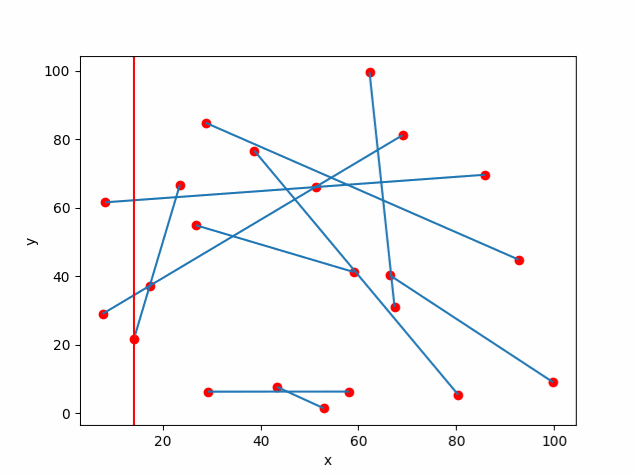
\includegraphics[width=0.8\linewidth]{4_1.png}
        \caption{Miotła w trakcie przejścia przez odcinki.}
    \end{figure}

    \subsection{Znajdowanie przecięć odcinków}
    Jeżeli miotła napotyka punkt, który jest przecięciem dwóch odcinków, zapisuje go
    do listy przecięć, która jest zwracana na końcu programu.

    \section{Analiza znalezionych przecięć odcinków}
    \subsection{Odcinki użyte do testów}

    \begin{figure}[H]
        \centering
        \begin{minipage}{0.45\linewidth}
          \centering
          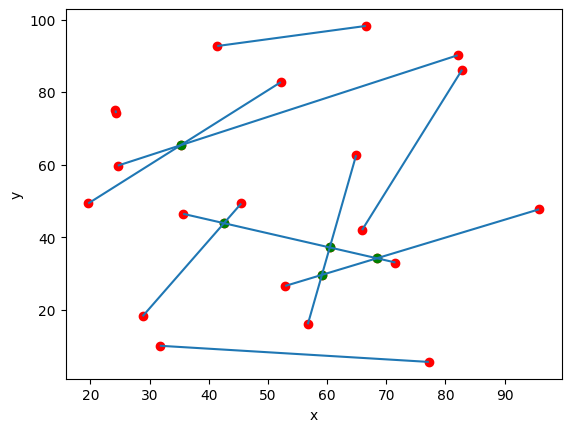
\includegraphics[width=1\linewidth]{4_2.png}
          \caption{}
        \end{minipage}
        \begin{minipage}{0.45\linewidth}
          \centering
          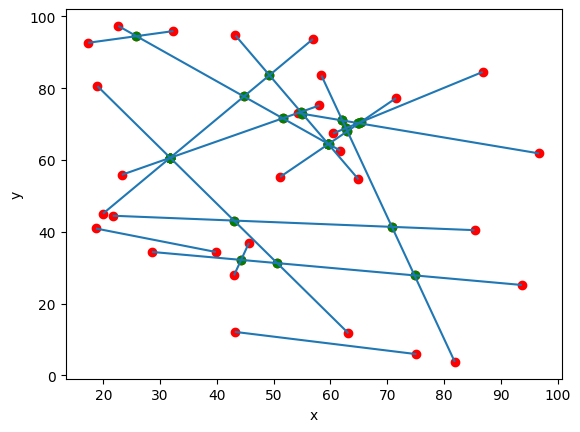
\includegraphics[width=1\linewidth]{4_3.png}
          \caption{}
        \end{minipage}
    \end{figure}

    \begin{figure}[H]
        \centering
        \begin{minipage}{0.45\linewidth}
          \centering
          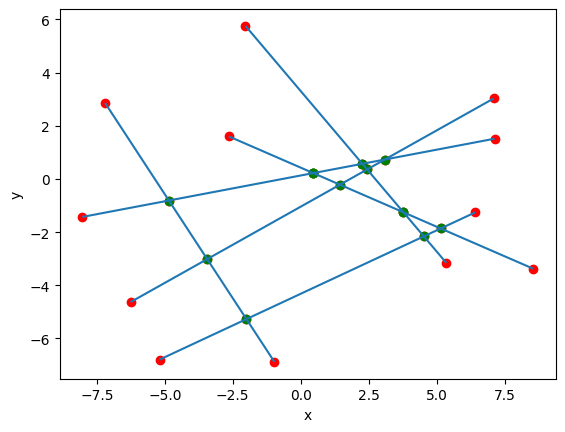
\includegraphics[width=1\linewidth]{4_4.png}
          \caption{}
        \end{minipage}
        \begin{minipage}{0.45\linewidth}
          \centering
          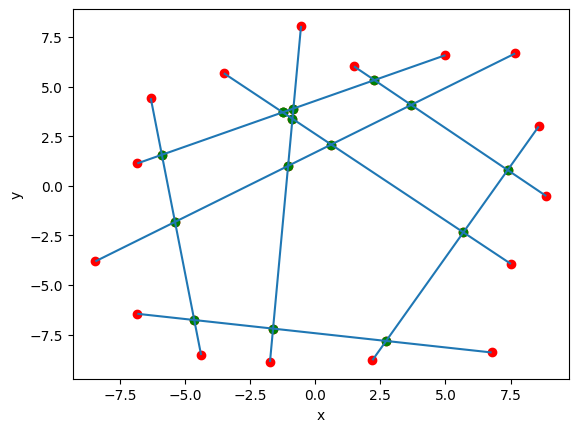
\includegraphics[width=1\linewidth]{4_5.png}
          \caption{}
        \end{minipage}
    \end{figure}

    \begin{figure}[H]
        \centering
        \begin{minipage}{0.45\linewidth}
          \centering
          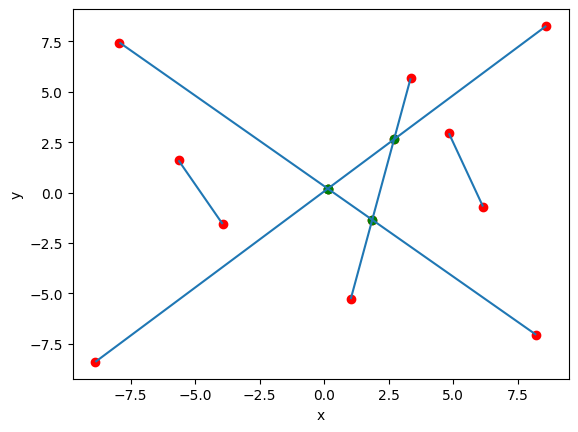
\includegraphics[width=1\linewidth]{4_6.png}
          \caption{}
        \end{minipage}
        \begin{minipage}{0.45\linewidth}
          \centering
          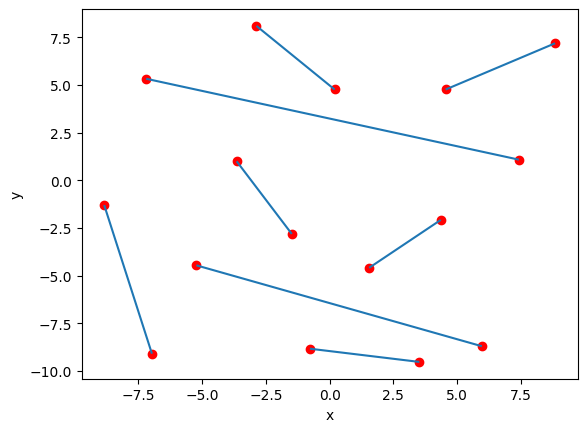
\includegraphics[width=1\linewidth]{4_7.png}
          \caption{}
        \end{minipage}
    \end{figure}

    \subsection{Analiza wyników}
    Rysunek 3 i rysynek 4 zawierają wygenerowane losowo odcinki, rysunek 4, rysunek
    5, rysunek 6 oraz rysunek 7 zostały wygenerowane ręcznie. Rysunek 7 nie zawiera
    żadnego przecięcia. Rysunek 4 i rysunek 5 zawierają wielokrotne przecięcia tych
    samych odcinków. Na rysunku 6 charakterystyczne są dwa krótkie odcinki, które
    nie przecinają się z żadnym innym, ale powodują pownowne sprawdzenie pozostałych
    odcinków. We wszystkich przypadkach algorytm działa poprawnie.

    \section{Wnioski}
    Algorytm dzięki swojej szybkości oraz uniwersalności jest dobrym narzędziem
    do znajdowania przecięć odcinków na płaszczyźnie. Jego złożoność obliczeniowa
    wynosi $O(nlogn)$, gdzie $n$ to liczba odcinków. Należy pamiętać, że uzyskanie
    takiej złożoności obliczeniowej wymaga użycia odpowiednich struktur danych
    pozwalających na szybkie aktualizacje i odczytywanie struktury zdarzeń
    i struktury stanu.

\end{document}
